\chapter{Design measurements}
\label{cha:measurements}
For measuring different simulation designs a example network was implemented using a monolithic and a modular design.
These implementations represent examples of the designs discussed in chapter \ref{cha:design}.
The simulation of this network using the different designs is used for analyzing the impact on the performance.


\section{Simulated example network}
\label{sec:measurements_network}
The example network simulates a message queue with different types of transmitted data (configuration, event, historical).
The different types of data are processed by different parts within the network.
This network includes parts for data generation and data processing.
Such a exemplary network was chosen, due to multiple similar practical applications.
An overview of the simulated network is shown in Figure \ref{fig:design_test_network}.

\begin{figure}
    \centering
    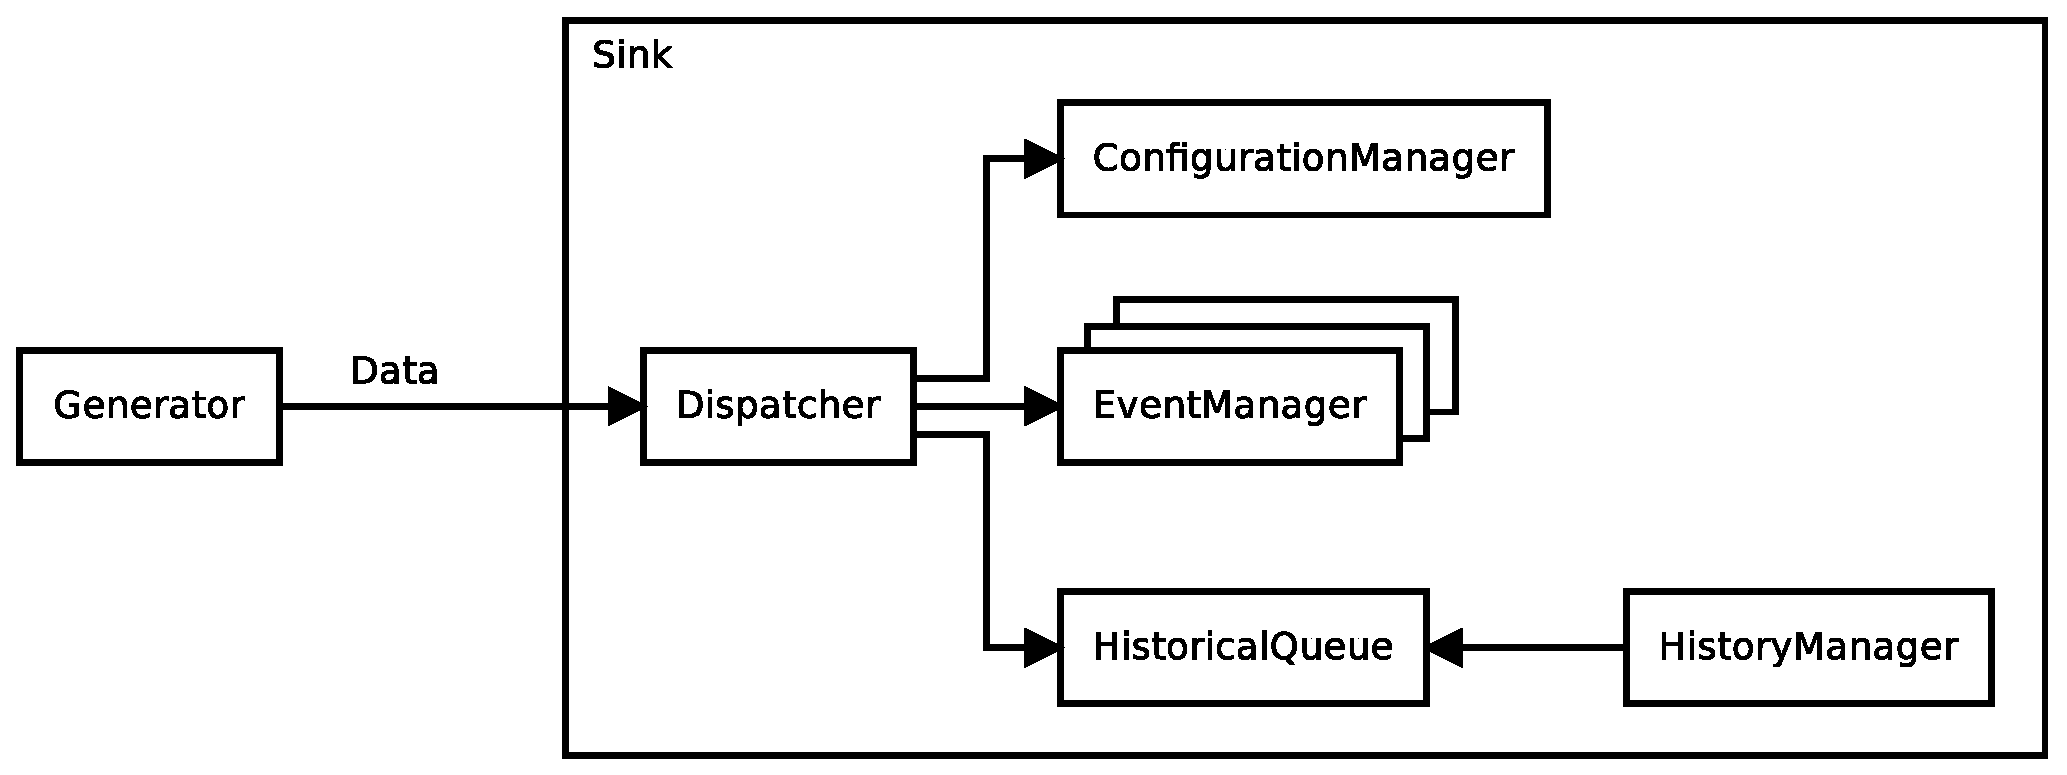
\includegraphics[width=0.9\linewidth]{design_test_network.eps}
    \caption{Example network including generator, sink, queue and different manager.}
    \label{fig:design_test_network}
\end{figure}

The \emph{Generator} generates cyclic data and a polling command.
Both are transmitted via messages to the sink module.
The generated data includes a field of 64 Bytes and a enumeration describing the type of data.
The generated polling command triggers the polling of the \emph{HistoryManager}.

These messages are transmitted to a sink, which is described via the interface module \emph{ISink}.
The differently designed modules \emph{ModularSink} and \emph{MonolithicSink} extend the interface and represent the different tested designs.

The first part within the sink is the \emph{Dispatcher} which is accessing the type information of the data and then forwards the packed data to the according parts.
Configuration and event data are forwarded to the \emph{ConfigurationManager} and the \emph{EventManager}.
These parts are simple implementations which executes various calculations on the received data to simulate processing.
Historical data are forwarded to the \emph{HistoricalQueue} which is internally implemented by a std::queue which holds all received data until they are accessed.
The \emph{HistoryManager} accesses the \emph{HistoricalQueue} and processes available data similar to \emph{ConfigurationManager} and \emph{EventManager} by executing dummy calculations.
This access is initiated by the generated polling commands from the \emph{Generator}.
\\

The functionality of dispatching and processing of the data is, as shown in Figure \ref{fig:design_test_network}, is included in the sink and is implemented twice with different designs.

The assumption of existing implementations for the \emph{Dispatcher}, \emph{ConfigurationManager}, \emph{EventManager} and \emph{HistoryManager} which must not be changed for the simulation is made.
Therefore implementing the \emph{MonolithicSink} consists of instantiating and connecting the different parts within a single simple module.
Received messages will be analyzed and the enclosed data or the polling command is forwarded to the according instances.

Implementing the \emph{ModularSink} requires the implementation of wrapper modules for every single part which should be represented by a separate module.
These wrapper extract the transmitted data of received messages and forward it to the enclosing parts.
Calls from within the enclosed parts are handled by methods of the wrappers, which are passed via function pointers (functional objects).
Within this methods according messages are created and sent via output gates.
The internal structure of the \emph{ModularSink} is shown in figure \ref{fig:ModularSink}.

\begin{figure}
    \centering
    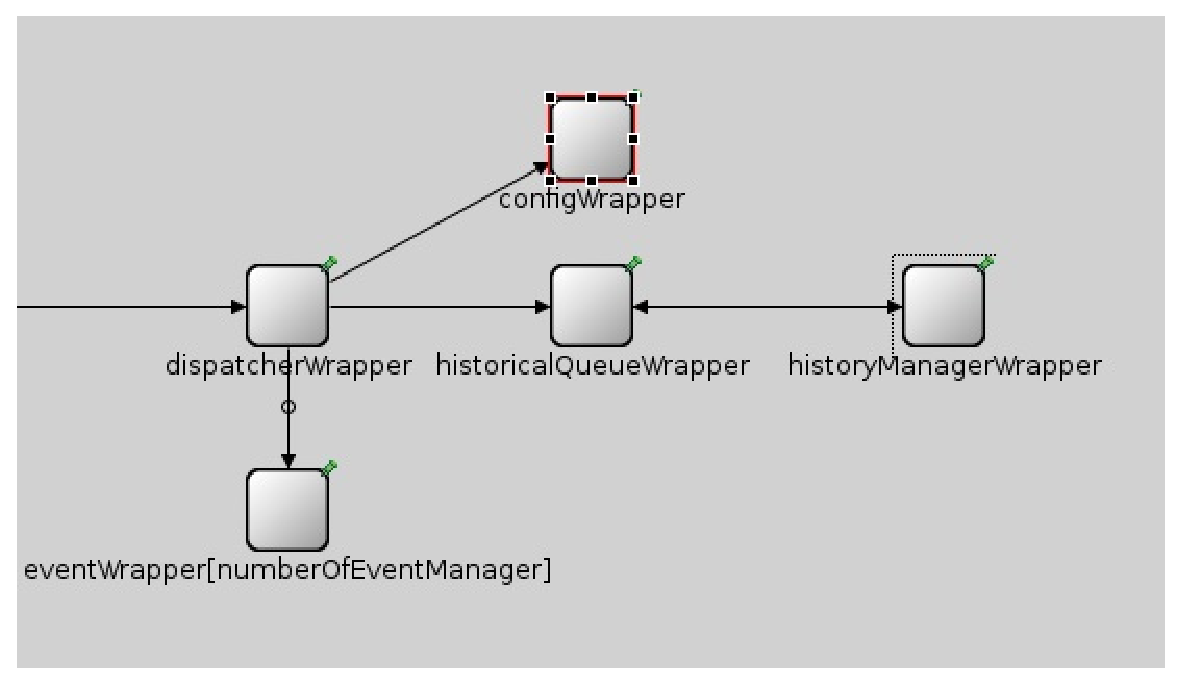
\includegraphics[width=0.9\linewidth]{images/ModularSink}
    \caption{Structure of \emph{ModularSink} showing the implemented Wrapper modules and their connections.}
    \label{fig:ModularSink}
\end{figure}

The simulated network is shown in figure \ref{fig:omnet_example_network}.
The \emph{Generator} instance is connected via two connections to the \emph{ISink} instance, although OMNeT++ only shows a single connection arrow.

\begin{figure}
    \centering
    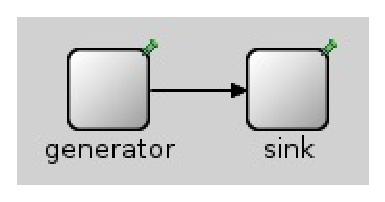
\includegraphics[width=0.3\linewidth]{images/omnet_example_network}
    \caption{Simulated example network showing the \emph{Generator} instance and its connection to the instance of the sink module derived from \emph{ISink}.}
    \label{fig:omnet_example_network}
\end{figure}

\section{Measurement methods}
\label{sec:measurements_methods}
For measuring the performance of the different designs three measurement methods were implemented.
These methods were implemented via different scripts for automated executing and designed dynamically allowing the analyze of various simulations and also either sequential or parallel simulation.

\subsection{Runtime measurement}
\label{sec:measurements_methods_runtime}
The performance of the simulated design can be analyzed by defining a fixed simulation time limit (\emph{sim-time-limit}).
Using the default (non real-time) scheduler this results in a simulation which executes as fast as possible for the needed number of event for reaching the simulation time limit.
The required time for this simulation represents the performance of the simulation.

Analyzing a parallel simulation using this method does not require special attention, except the handling of multiple resulting runtime values.

\subsection{Processed event count}
\label{sec:measurements_methods_event}
By defining a fixed execution time limit (\emph{cpu-time-limit}) and using the default scheduler the simulation will run for a fixed time.
The number of processed events within this fixed time represents the performance of the simulation.

The simulation of different designs results in contrasting event counts due to the increased number of messages within a modular design.
Therefore for evaluating the created number within a fixed processing time the ratio of event creation must be determined.
This ratio can be measured using the previous method \ref{sec:measurements_methods_runtime}.

Such a ratio or offset must also be considered for the analyze of parallel simulations due to the increased number of messages for synchronization.
This correction values can also be determined using the previous method \ref{sec:measurements_methods_runtime}.
The impact of synchronization within parallel simulations is described in section \ref{sec:parallel_omnet_sync}

\subsection{Real time behavior}
\label{sec:measurements_methods_realtime}
Using the built in real time scheduler \emph{cRealTimeScheduler} the simulation will try to execute the simulation matching the real time.
The performance output (\emph{cmdenv-performance-display}) provides the ratio of simulated seconds per real second.
As described in section \ref{sec:simulation_omnet} this ratio must not differ too much from one for representing a real-time simulation.
The simulated network provides a configurable interval of data/command generation.
Using a parameter study (described in section \ref{sec:omnet_running_config}) the interval for data/command generation can be set with values form a range of intervals.
With attention to the performance ratio of the different iterations the interval limit, which still allows real-time simulation, can be determined.

\subsection{Result recording}
The results of the different measurement methods are all extracted from the resulting command line output of the simulation.
The automated test scripts are analyzing the outputs of the executed simulation after finishing the simulation.
For preventing the delay of the measurements and the simulation by writing the output to a file located on an slow peripheral the output files are located on a \emph{ramdisk}.
A \emph{ramdisk} represents a filesystem which is located within the \emph{RAM} (Random access memory) and therefore provides the maximum speed for writing and analyzing outputs.

\section{Sequential Simulation}
\label{sec:measurements_sequential}
The implemented test network described in \ref{sec:measurements_network} was developed and analyzed on a Lenovo ideapad U530 with 8GB PC3-12800 DDR3 SDRAM 1600 MHz and a 4th Gen Intel® Core™ i7-4500U (1.8 GHz 200 MHz 4MB) running Kubuntu 15.10.
\cite{lenovo_spec}

%TODO: find correct place for specs and add APC spec and execute simulation on APC

\begin{figure}
    \centering
    \pgfplotsset{
        every axis plot/.append style={very thick}
    }
    \begin{tikzpicture}
 %       \begin{axis}[
 %       ylabel={Runtime $[ns]$},
%        xlabel={Simulation time $[ns]$},
%        grid=major,
%        legend entries={Modular,Monolithic}
%        ]
%        
%        \addplot[dotted,
%        discard if not={Configuration}{Modular}] table {
%            Prefix Configuration Parameter
%            1s Modular 0.051s
%            1s Monolithic 0.009s
%            2s Modular 0.052s
%            2s Monolithic 0.017s
%            5s Modular 0.124s
%            5s Monolithic 0.046s
%            10s Modular 0.252s
%            10s Monolithic 0.083s
%            20s Modular 0.543s
%            20s Monolithic 0.167s
%            50s Modular 1.225s
%            50s Monolithic 0.416s
%            100s Modular 2.451s
%            100s Monolithic 0.831s
%            200s Modular 4.924s
%            200s Monolithic 1.648s
%            500s Modular 12.211s
%            500s Monolithic 4.210s
%            1min Modular 1.478s
%            1min Monolithic 0.499s
%            2min Modular 2.969s
%            2min Monolithic 1.040s
%            5min Modular 7.387s
%            5min Monolithic 2.519s
%            10min Modular 14.607s
%            10min Monolithic 4.986s
%            20min Modular 29.257s
%            20min Monolithic 11.775s
%            30min Modular 43.866s
%            30min Monolithic 14.982s
%            };
%        \end{axis}
    \end{tikzpicture}    
    \caption{Runtime results for different designs over different simulation time limits.}
    \label{fig:results_runtime_sim_time}
\end{figure}




\begin{table}
    \centering
    \begin{tabular}{|c|c|c|c|}
        \hline \textbf{Design} & \textbf{Runtime} & \textbf{Event} & \textbf{Real-time} \\
        \hline 
        \hline Modular & 1234 & 5678 & 9012 \\ 
        \hline Monolithic & 1234 & 5678 & 9012  \\ 
        \hline 
    \end{tabular}
    \label{tab:measurements_design_seq}
    \caption{Different performance results for different designs.}
    
\end{table}

\section{Parallel simulation}
\label{sec:measurements_parallel}